\chapter{Introduction}
\label{chap:1}
\noindent Chapter~\ref{chap:1} gives a general introduction to the thesis contributions. Section~\ref{sec:m} describes Distributed Ledger Technology and points out the main issue this area is facing now. Section~\ref{sec:r} lists out the main problem this thesis addresses. This is followed by the discussion of the research methods, objectives and delimitations in Section~\ref{sec:rm},~\ref{sec:ro}, and \ref{sec:d}. The outline of the thesis is presented in Section~\ref{sec:to}. 

\section{Motivation}
\label{sec:m}

\noindent Initially, the ledger means the foundation of accounting. However, it is not difficult to find that there are many shortcomings in the long-term use of traditional ledgers, for example, low efficiency, high cost, opacity and easy to cause fraud and abuse issues~\cite{versus}.\\

\noindent With the development of information technology, these ledgers have gradually evolved into digital technology. The distributed ledger is a significant leap after the digitization of ledger-based technology. It is a database that is shared, replicated, and synchronized between network members~\cite{brakeville2016blockchain}. It records transactions between network participants, such as the exchange of assets or data. From a technical point of view, the Distributed Ledger Technology (DLT) not only inherits the traditional bookkeeping philosophy but also has its unique innovations, which has some advantages that traditional ledgers cannot reach.\\

\noindent Blockchain systems perform as one "single-machine" for a long time since the Bitcoin was introduced. Every blockchain is highly independent and challenging to communicate with each other. Hence, the data and services in the blockchain world are confined to the individual blockchain. As a result, this phenomenon will discourage development. As if we could find a standardized cross-chain protocol/platform that could link all blockchain systems, the services could be more specific and complete due to the co-operation of the blockchains. The popularization and maturity of cross-chain technology will lead a revolutionary development in the blockchain field. Moreover, different from the Internet to achieve the circulation of information, cross-ledger could realize the distribution of values.\\

\noindent Based on the background above, there exist many distributed ledgers, but for them to be fully distributed, there is a strong need of them to communicate with each other and also traditional ledgers. Otherwise, the consistency between the ledgers of different entities across the chain would not be guaranteed. There have been many different approaches, such as cross-chain protocols and platforms released to realize the cross-chain transactions, so it is worthy of finding out the differences between them.

\section{Research Questions}
\label{sec:r}
\noindent There is one technical issue that affects the blockchain developers, which is the \textit{\textbf{intercommunications}}. A single blockchain network is a relatively closed system that does not actively interact with the outside world. The assets of each chain are also an independent value system. If we can break through the interoperability among different ledgers and let the value circulate on the broader world, it will inevitably promote the rapid development of the blockchain industry. Cross-chain technology is dedicated to building a bridge of trust between ledgers, breaking the situation of an isolated value system, and realizing asset interoperability to achieve a real win-win situation.\\

\noindent For the existing blockchain system, it is very \textbf{time-consuming} and \textbf{laborious} to connect them individually. With the development of the computer network, we need a set of across chain standards for blockchain interoperability, but this is not an easy thing to do. It should be an industry-driven standard that is widely applied. When the majority of projects follow a common, easy-to-use protocol, this standard is genuinely established. Having a universal standard of cross-chain communication patterns can be represented as an important milestone for the industry. The rapid flow of information will inevitably drive the improvement of efficiency and become the internal driving force for the development of the blockchain industry.\\


\noindent In fact, cross-chain technology is facing several key difficulties such as how to ensure atomicity, etc. The detailed discussion is elaborated in section ~\ref{sec:diff}. So how well a mature cross-chain project meets with those criteria will be taken into consideration during the whole study.
\\

\section{Research Methodology}
\label{sec:rm}
\noindent This project mainly makes uses of a combination of qualitative and quantitative research strategy.\\

\noindent For the beginning of this research, a literature study and review was taken first to gain a deep understanding of cross-ledger history and realization of communications through published papers. Then the critical point is the case study among popular projects. By studying the different cross-chain implementations, exacting the ideas and scheme they uses, we can summarize and categorize them into different groups, hence, identify patterns and commonalities in the cross-chain field. Moreover, we can help the increasing developers to consummate the blockchain design.\\

\noindent To gain a proper perspective of the practical usage and performance of purposed solutions, it is necessary to actually implement at least one of them.  During this thesis, we introduced two test cases at the implementation stage, involving theoretical comparison between a framework design and integration with the HTLC atomic swaps, and one asset transfer test scenario working mechanism analysis.  
         
\section{Research Objectives}
\label{sec:ro}
\noindent My research has contributed to the universal demanding and requirements on cross-ledger communication towards blockchain areas. In particular, I have focused on the problems that the realization of cross-chain communication is facing.\\

\noindent To understand different patterns or implementations of cross-chain technology, we need to start with the history of cross-chain and grasp the \textbf{main idea of chain interoperability} based on literature review. Based on those findings, we summarized the fundamental problems the blockchains are facing, according to those difficulties, I will give several examples through the case study in the following chapters.  The \textbf{analysis and comparison} from various aspects will next lead to a standard and universal needs of the cross-chain area. In my thesis, I have considered the following three major elements of this study as shown in Figure \ref{fig:contri}

    \begin{figure}[H]
    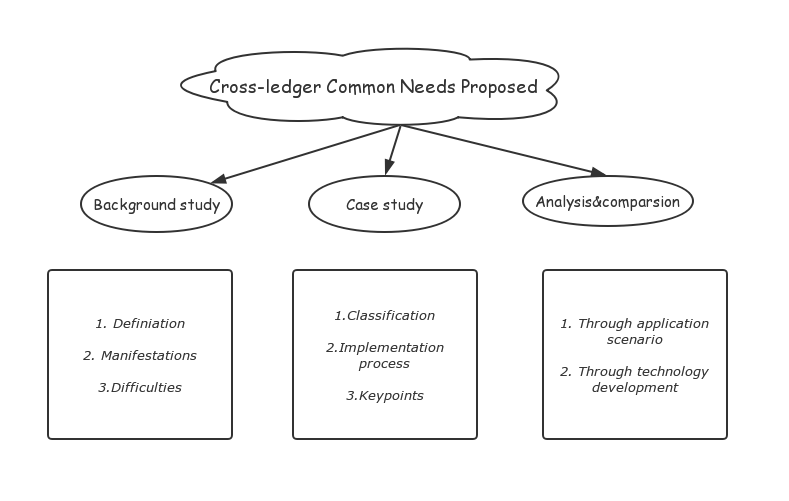
\includegraphics[width=0.8854\textwidth]{./figures/contri.png}
    \centering
    \caption{Research components of cross-chain intercommunication}%\protect\footnotemark}
    \centering
    \label{fig:contri}
    \end{figure}


\section{Delimitations}
\label{sec:d}
\noindent Information provided in this thesis work is the result of multiple new kinds of research, some findings and theoretical background are based on publicly available resources of varying quality, including the posts from the discussion forum. Addressing the cross-chain problem located in one specific field could lead to an unbalanced view, since cross-chain may evolve into a financial aspect that I do not comprehend. This thesis conclusion does not provide any suggestion for investment.\\

\noindent There are tons of nuance, variations in cross-chain system design and assumptions. Due to the time limit, here we focus on the analysis of specific cross-chain transactions performance. Aside from the projects that are not landing for use, many projects outlined are proposing solutions that in requirement of multiple different blockchain systems, so we are not able to test them out accordingly.

\section{Thesis Organization}
\label{sec:to}
This thesis is organized into five chapters, as follows:

$\bullet $ Chapter \ref{chap:1} concentrates on the research value and market meaning of this thesis, then briefly introduces the concept of cross-chain communication.

$\bullet $ Chapter \ref{chap:2} studies the background of the cross-chain project by classifying different manifestations of cross-chain communication as well as pointing out the problems cross-ledger communication are facing.

$\bullet $ Chapter \ref{chap:3} focuses on the theoretical solutions that will address the difficulties, discusses the communication process of various cross-chain projects based on different group rules. 

$\bullet $ Chapter \ref{chap:4} puts efforts in analyzing the market demand situation, and discusses the applications that could be adopted. Besides, this chapter also compares the technology development of some representative projects.

$\bullet $ Chapter \ref{chap:5} summarizes the findings during the research and suggests several ideas for related future work.

$\bullet $ \nameref{app:A} contains a comparison table that evaluates 20 cross-chain projects from several valuable aspects.

$\bullet $ \nameref{app:B} lists implementation code pieces with essential functions explained and the utilization of smart contracts, for further test usage.
  